\only<1>{
    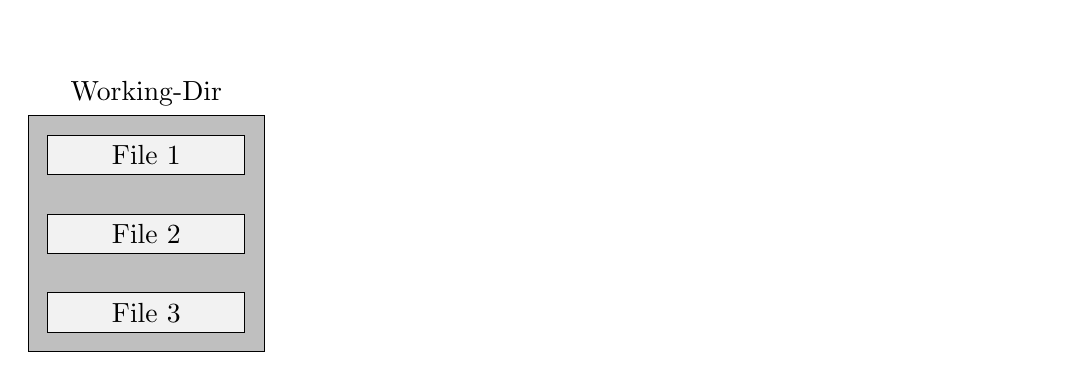
\begin{tikzpicture}
        \filldraw[draw=black, fill=gray!50] (0,0) rectangle (3,3);

        \node[above]() at (1.5, 3){Working-Dir};

        \filldraw[draw=black, fill=gray!10] (0.25,2.25) rectangle (2.75,2.75) node() [pos=.5] {File 1};
        \filldraw[draw=black, fill=gray!10] (0.25,1.25) rectangle (2.75,1.75) node() [pos=.5] {File 2};
        \filldraw[draw=black, fill=gray!10] (0.25,0.25) rectangle (2.75,0.75) node() [pos=.5] {File 3};
        \node() at(13,4){};
    \end{tikzpicture}
}

\only<2>{
    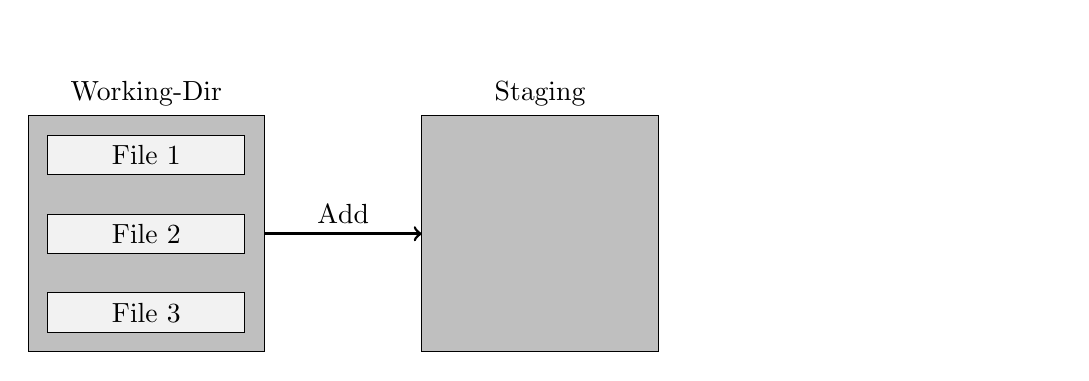
\begin{tikzpicture}
        \filldraw[draw=black, fill=gray!50] (0,0) rectangle (3,3);
        \filldraw[draw=black, fill=gray!50] (5,0) rectangle (8,3);

        \node[above]() at (1.5, 3){Working-Dir};
        \node[above]() at (6.5, 3){Staging};

        \draw[line width=1pt, ->] (3, 1.5) -- (5,1.5) node[midway, above]() {Add};

        \filldraw[draw=black, fill=gray!10] (0.25,2.25) rectangle (2.75,2.75) node() [pos=.5] {File 1};
        \filldraw[draw=black, fill=gray!10] (0.25,1.25) rectangle (2.75,1.75) node() [pos=.5] {File 2};
        \filldraw[draw=black, fill=gray!10] (0.25,0.25) rectangle (2.75,0.75) node() [pos=.5] {File 3};
        \node() at(13,4){};
    \end{tikzpicture}
}

\only<3>{
    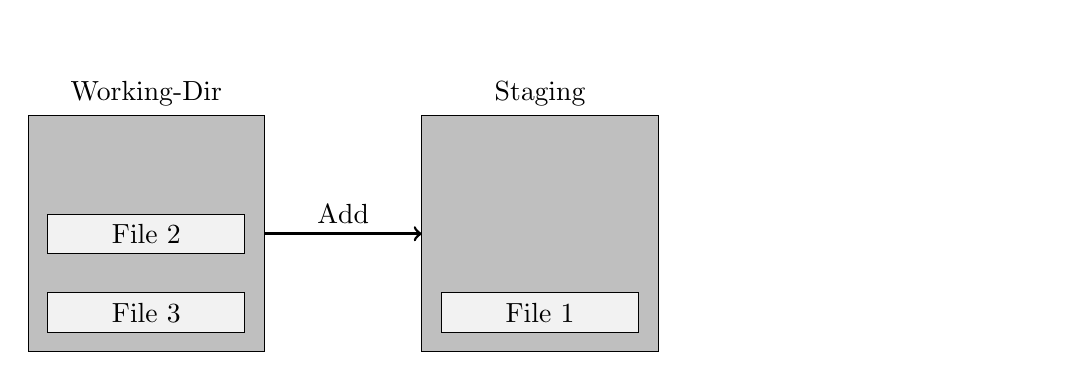
\begin{tikzpicture}
        \filldraw[draw=black, fill=gray!50] (0,0) rectangle (3,3);
        \filldraw[draw=black, fill=gray!50] (5,0) rectangle (8,3);

        \node[above]() at (1.5, 3){Working-Dir};
        \node[above]() at (6.5, 3){Staging};

        \draw[line width=1pt, ->] (3, 1.5) -- (5,1.5) node[midway, above]() {Add};

        \filldraw[draw=black, fill=gray!10] (0.25,0.25) rectangle (2.75,0.75) node() [pos=.5] {File 3};
        \filldraw[draw=black, fill=gray!10] (0.25,1.25) rectangle (2.75,1.75) node() [pos=.5] {File 2};
        \filldraw[draw=black, fill=gray!10] (5.25,0.25) rectangle (7.75,0.75) node() [pos=.5] {File 1};
        \node() at(13,4){};
    \end{tikzpicture}
}

\only<4>{
    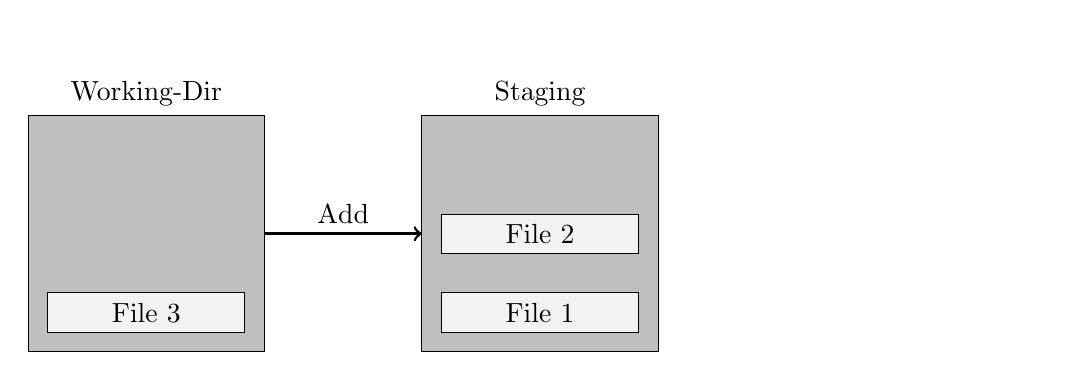
\begin{tikzpicture}
        \filldraw[draw=black, fill=gray!50] (0,0) rectangle (3,3);
        \filldraw[draw=black, fill=gray!50] (5,0) rectangle (8,3);

        \node[above]() at (1.5, 3){Working-Dir};
        \node[above]() at (6.5, 3){Staging};

        \draw[line width=1pt, ->] (3, 1.5) -- (5,1.5) node[midway, above]() {Add};

        \filldraw[draw=black, fill=gray!10] (0.25,0.25) rectangle (2.75,0.75) node() [pos=.5] {File 3};
        \filldraw[draw=black, fill=gray!10] (5.25,1.25) rectangle (7.75,1.75) node() [pos=.5] {File 2};
        \filldraw[draw=black, fill=gray!10] (5.25,0.25) rectangle (7.75,0.75) node() [pos=.5] {File 1};
        \node() at(13,4){};
    \end{tikzpicture}
}

\only<5>{
    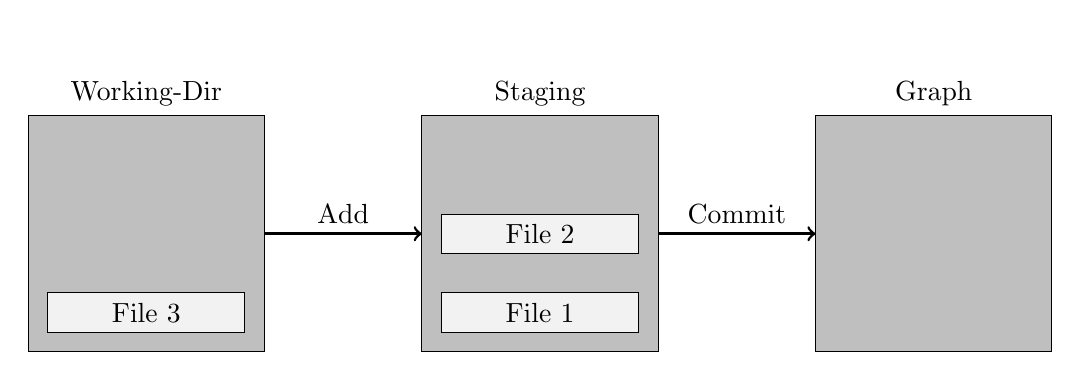
\begin{tikzpicture}
        \filldraw[draw=black, fill=gray!50] (0,0) rectangle (3,3);
        \filldraw[draw=black, fill=gray!50] (5,0) rectangle (8,3);
        \filldraw[draw=black, fill=gray!50] (10,0) rectangle (13,3);

        \node[above]() at (1.5, 3){Working-Dir};
        \node[above]() at (6.5, 3){Staging};
        \node[above]() at (11.5, 3){Graph};

        \draw[line width=1pt, ->] (3, 1.5) -- (5,1.5) node[midway, above]() {Add};
        \draw[line width=1pt, ->] (8, 1.5) -- (10,1.5) node[midway, above]() {Commit};

        \filldraw[draw=black, fill=gray!10] (0.25,0.25) rectangle (2.75,0.75) node() [pos=.5] {File 3};
        \filldraw[draw=black, fill=gray!10] (5.25,1.25) rectangle (7.75,1.75) node() [pos=.5] {File 2};
        \filldraw[draw=black, fill=gray!10] (5.25,0.25) rectangle (7.75,0.75) node() [pos=.5] {File 1};
        \node() at(13,4){};
    \end{tikzpicture}
}

\only<6>{
    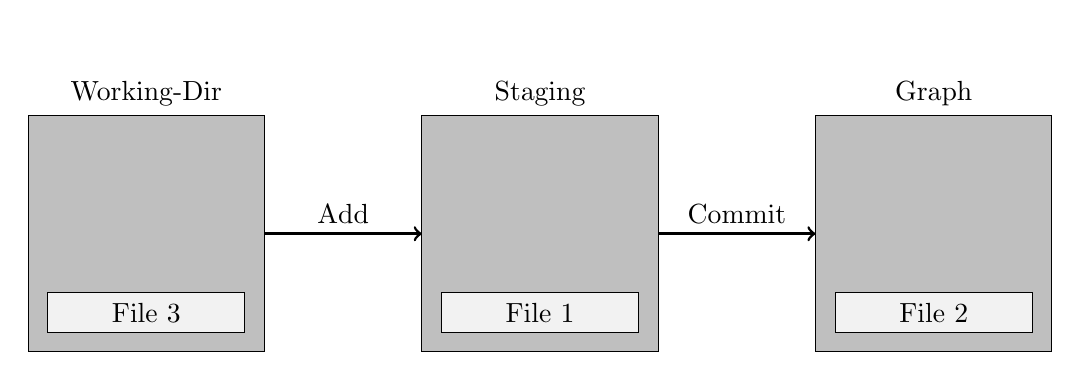
\begin{tikzpicture}
        \filldraw[draw=black, fill=gray!50] (0,0) rectangle (3,3);
        \filldraw[draw=black, fill=gray!50] (5,0) rectangle (8,3);
        \filldraw[draw=black, fill=gray!50] (10,0) rectangle (13,3);

        \node[above]() at (1.5, 3){Working-Dir};
        \node[above]() at (6.5, 3){Staging};
        \node[above]() at (11.5, 3){Graph};

        \draw[line width=1pt, ->] (3, 1.5) -- (5,1.5) node[midway, above]() {Add};
        \draw[line width=1pt, ->] (8, 1.5) -- (10,1.5) node[midway, above]() {Commit};

        \filldraw[draw=black, fill=gray!10] (0.25,0.25) rectangle (2.75,0.75) node() [pos=.5] {File 3};
        \filldraw[draw=black, fill=gray!10] (5.25,0.25) rectangle (7.75,0.75) node() [pos=.5] {File 1};
        \filldraw[draw=black, fill=gray!10] (10.25,0.25) rectangle (12.75,0.75) node() [pos=.5] {File 2};
        \node() at(13,4){};
    \end{tikzpicture}
}
